% ================================================================= 11b
\section{Results on BEAM}\label{sec:beam}

\begin{table}[!htb]
\centering\small
\setlength{\tabcolsep}{4pt}
\begin{tabular}{@{}l c c c r r@{}}
\toprule
\thead{System} & \theadm{Contra-\\diction (40)} & \theadm{Update\\(40)} & \theadm{Both (80)\\95\% CI} & \theadm{\mx{} wins\\/ losses} & \theadm{Memory\\tokens}\\
\midrule
\mx{} ranked (4k) & \best{66.2} & 53.8 & \best{60.0} [51, 68] & -- & \best{897}\\ \rowrule
mem0 top-30 & 55.6 & 51.9 & 53.8 [45, 62] & 29 / 15, $p=0.049$ & 1,932\\ \rowrule
full context & 46.6 & \best{61.3} & 53.9 [45, 63] & 27 / 14, $p=0.06$ & 175,931\\ \rowrule
chunk RAG (4k) & 45.9 & 45.6 & 45.8 [37, 54] & 35 / 14, $p=0.004$ & 3,958\\
\bottomrule
\end{tabular}
\caption{\textbf{BEAM-100K, 20 conversations, 80 questions; BEAM's rubric judge (\%).} Haiku 5.5 extraction and
answering. Bootstrap 95\% intervals; wins / losses count questions where \mx{} scored higher / lower (two-sided sign
test).}
\label{tab:beam}
\end{table}

\begin{figure}[!htb]
\centering
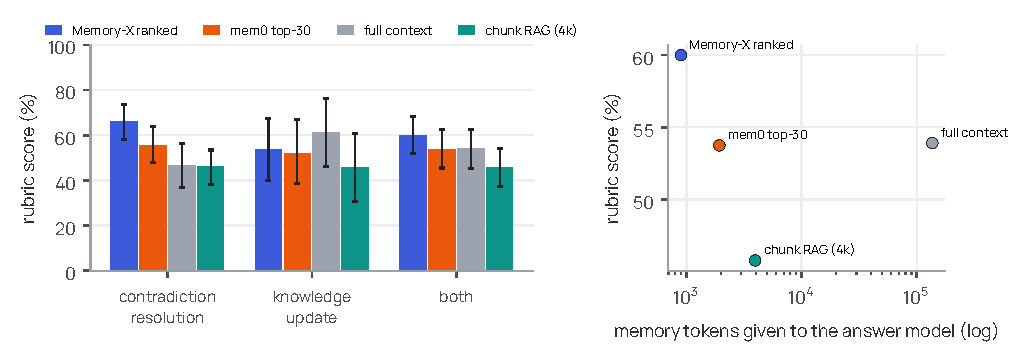
\includegraphics[width=\linewidth]{figures/fig_beam.pdf}
\caption{\textbf{BEAM rubric score by ability} (left, bootstrap 95\% intervals) and \textbf{against the size of the
memory block} (right, log scale).}
\label{fig:beam}
\end{figure}

\mx{} scored highest overall (60.0\%) with the smallest block: \textbf{897 tokens, 2.2 times fewer than mem0} (53.8\%)
and 196 times fewer than full context (53.9\%). Against mem0 it won 29 questions and lost 15 ($p=0.049$). The gain is
in \textbf{contradiction resolution}: 66.2\% against 55.6\% (22 wins, 9 losses, $p=0.029$). These questions reward
naming both sides of a conflict. Because a replacement needs $P\ge0.9$, an incompatible pair Jev is unsure about stays
as two related, dated facts, and the answering model sees both: 28 of \mx{}'s 40 answers flagged the contradiction,
against 20 for mem0 and 20 for full context. On \textbf{knowledge updates} \mx{} and mem0 were level (53.8\% and
51.9\%), and full context did best (61.3\%).

Ingesting the 20 conversations cost \mx{} \$0.136 per conversation (extraction \$0.053, Jev \$0.083). In mem0, 97
extraction responses could not be parsed and stored nothing; we left that behaviour as shipped.
